\documentclass{standalone}

\usepackage{tikz}
\usetikzlibrary{math}

\begin{document}
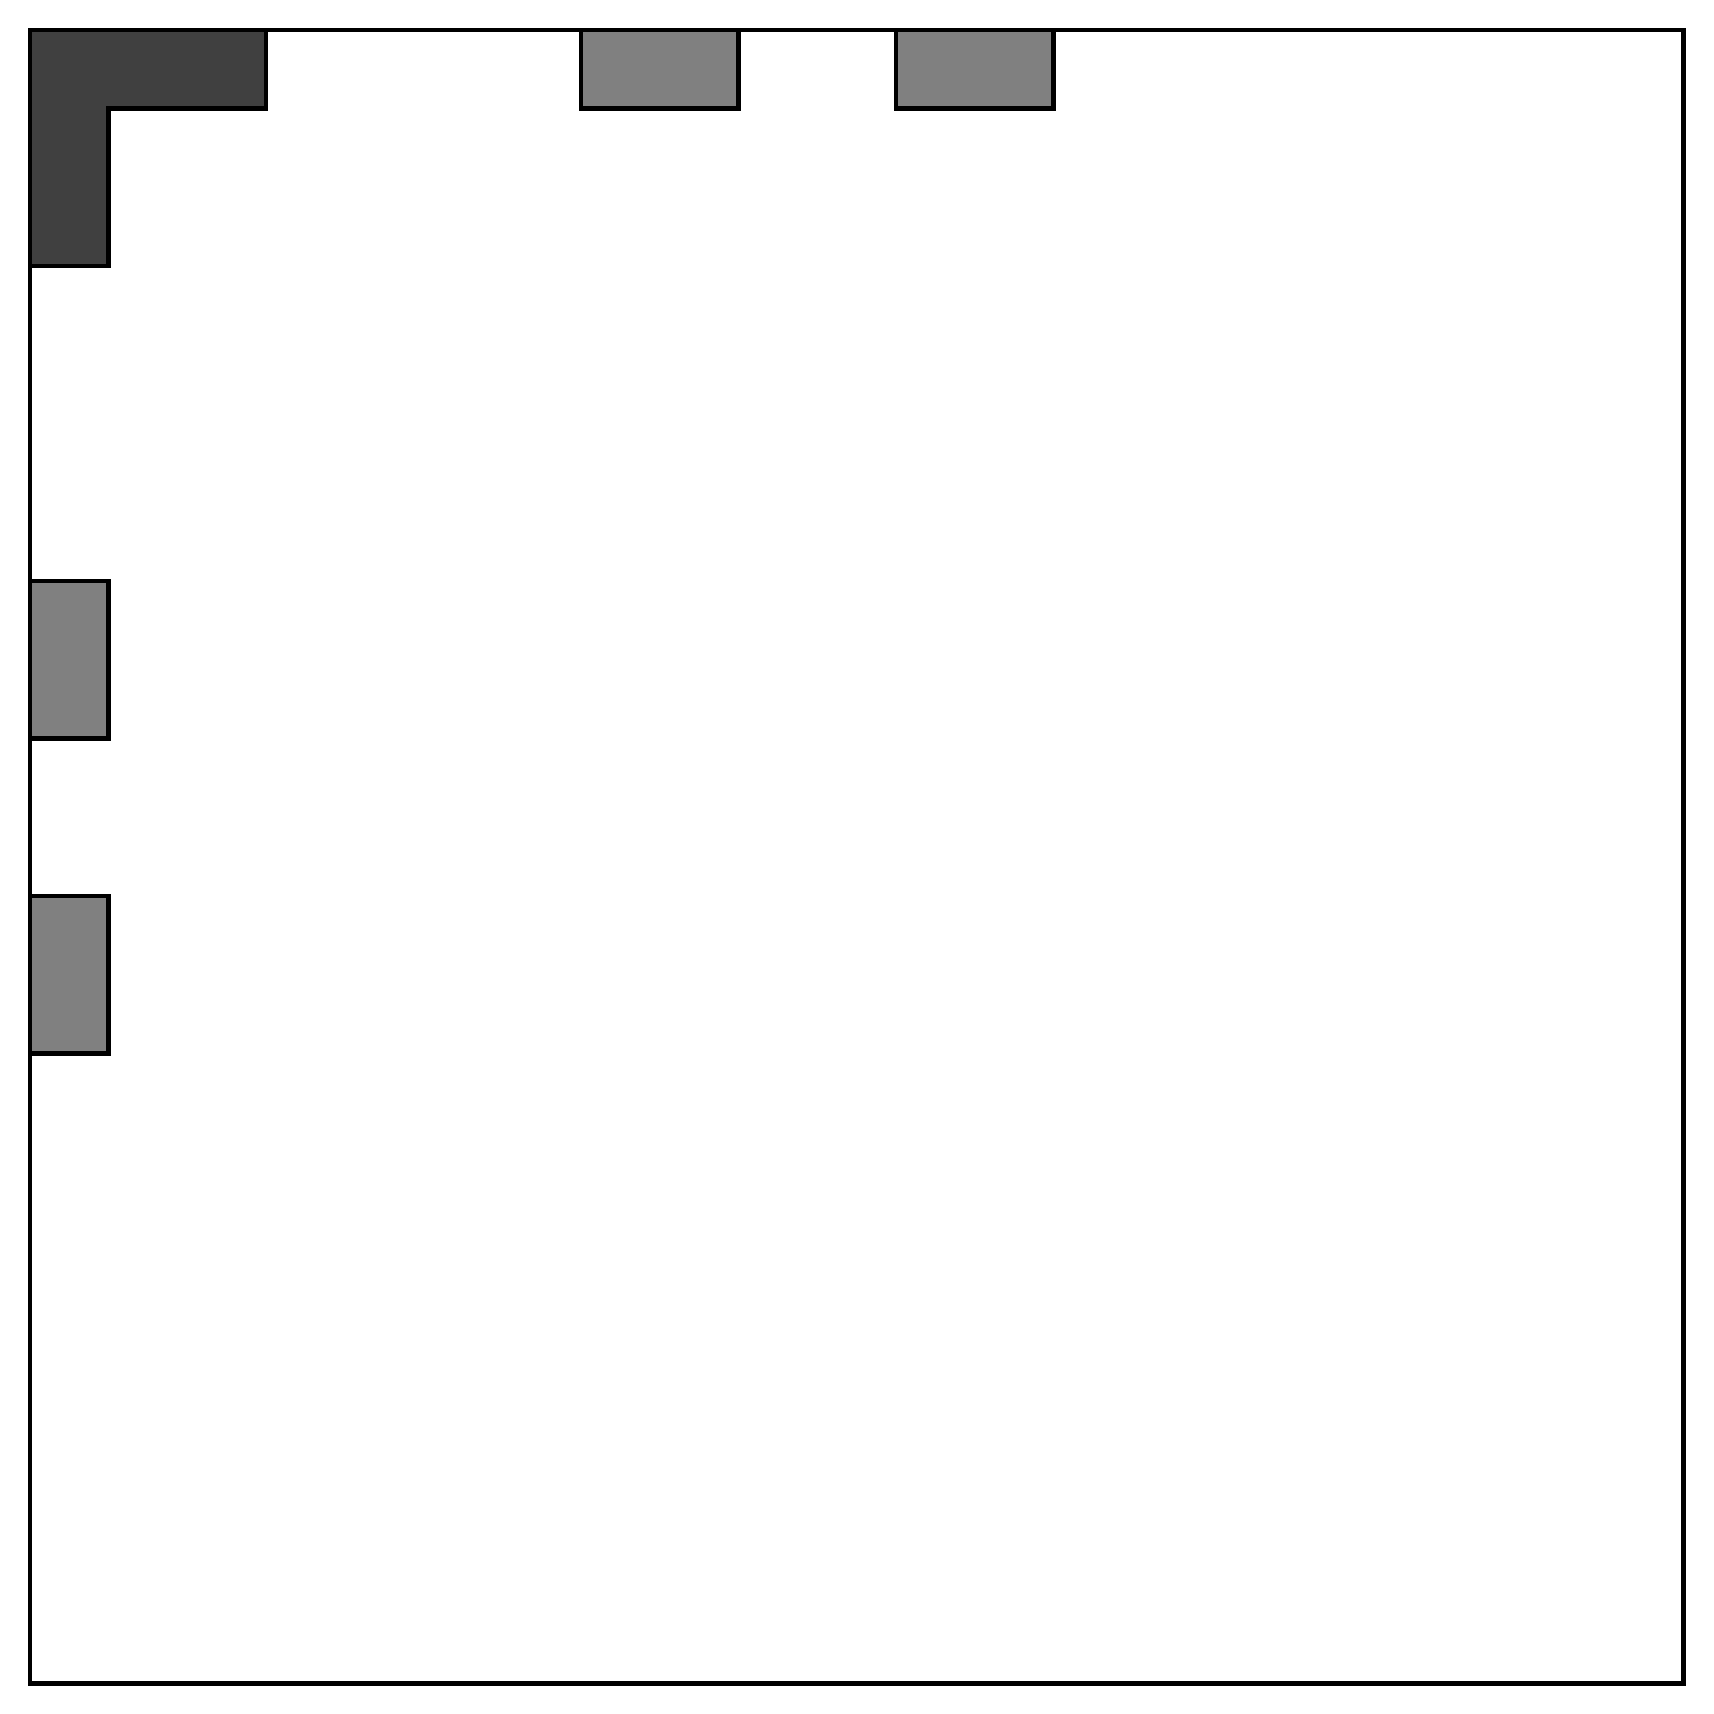
\begin{tikzpicture}
  \tikzmath{\m = 21;}
  \tikzmath{\i = 2;}
  \tikzmath{\j = 4;}

  \draw[ultra thick] (0, 0) rectangle ++(\m, \m);

  \path [draw, ultra thick, fill=darkgray] (0, \m-3) -- (1, \m-3) -- (1, \m-1) -- (3, \m-1)
    -- (3, \m) -- (0, \m) -- (0, \m-3);

  \draw[ultra thick, fill=gray] (3+2*\i, \m-1) rectangle ++(2, 1);
  \draw[ultra thick, fill=gray] (0, \m-3-2*\i-2) rectangle ++(1, 2);
  
  \draw[ultra thick, fill=gray] (3+2*\j, \m-1) rectangle ++(2, 1);
  \draw[ultra thick, fill=gray] (0, \m-3-2*\j-2) rectangle ++(1, 2);
\end{tikzpicture}
\end{document}